\chapter{Finding The Best Model}
\label{ch:finding-the-best-model}

\begin{keytakeaway}
    In this chapter we test all models outlined in the Methods chapter to assess their accuracy, understand their strengths and weaknesses, and identify the most important features to forecast decarbonization. We find that, in terms of accuracy, \textbf{CatBoost} is the best model for this dataset, showcasing marginally better results on the test set compared to all other models. Overall, our results suggest that \textbf{Mixed Effects Model} is the ideal model for uncovering key relationship between predictors and future decarbonization rates. Most importantly, we find that \textbf{different models identify similar sets of important features}, confirming the hypothesis that from the CDP survey we can identify a group of key variables that together are most indicative of next-year decarbonization rate.
\end{keytakeaway}



\section{Modeling Roadmap}
In this chapter, we will tune, benchmark, and report the results of various models to forecast next year's real decarbonization rate. Our goal is to inform industry stakeholders on the predictive capabilities of the CDP survey and, at the same time, to determine the most important features predictive of future decarbonization.

We will test the following models: Mixed Effects Model from Chapter 5, Bayesian Ridge Regressor, CatBoost Regressor, Ridge Regression, Orthogonal Matching Pursuit, Elastic Net, Lasso Regression, Lasso Least Angle Regression, Gradient Boosting, Random Forest, Light Gradient Boosting Machine, Extra Trees, Dummy Regressor, Extreme Gradient Boosting, K Neighbors Regressor, Huber Regressor, Decision Tree, AdaBoost, Passive Aggressive Regressor, and Ordinary Least Squares. Benchmarking for all models is facilitated through the Pycaret library \cite{pycaret}. 

As a first step, we will be re-training the final mixed-effects model (30), which is outlined in the preceding chapter, Table \ref{tab:R10}. Then, model (30) will be compared to all other models which include a range of more adaptive, data-centric non-parametric methodologies. We will be evaluating the predictions based on Root Mean Squared Error (RMSE), Mean Absolute Error (MAE), and R-squared \cite{gmd} with respect to the test set. 

Then, the body of the chapter is dedicated to exploring and refining the three models introduced in the Methods chapter, which I believe to be the most promising: the Mixed Effects Model, Bayesian Ridge, and CatBoost Regressor. For a detailed methods description of all other models used for benchmarking, please refer to Pycaret's and Sklearn's documentation \cite{pycaret,scikit-learn}.

% Initially, our approach involves retraining the mixed-effects model (30), as outlined in the preceding chapter and detailed in Table \ref{tab:R10}. Subsequently, this model will be compared with a range of more adaptive, data-centric non-parametric methodologies, including decision trees and various ensemble strategies. The evaluation criteria for these models will encompass the Root Mean Squared Error (RMSE), Mean Absolute Error (MAE), and the R-squared metric \cite{gmd}. The models subjected to assessment in this segment include the Mixed Effects Model from Chapter 5, Bayesian Ridge Regressor, CatBoost Regressor, Ridge Regression, Orthogonal Matching Pursuit, Elastic Net, Lasso Regression, Lasso Least Angle Regression, Gradient Boosting, Random Forest, Light Gradient Boosting Machine, Extra Trees, Dummy Regressor, Extreme Gradient Boosting, K Neighbors Regressor, Huber Regressor, Decision Tree, AdaBoost, Passive Aggressive Regressor, and Ordinary Least Squares. Benchmarking for all models is facilitated through the Pycaret library \cite{pycaret}. The core focus of this chapter is devoted to the in-depth exploration and enhancement of three models introduced in the Methods section, which are deemed to be particularly promising: the Mixed Effects Model, Bayesian Ridge, and CatBoost Regressor. For comprehensive methodological details on the remaining models utilized for benchmarking purposes, readers are directed to consult the documentation provided by Pycaret and Sklearn \cite{pycaret,scikit-learn}.

\subsection{Data Preprocessing}
The predictors in this chapter are the same as the ones analyzed across all Chapter 5 models, but the data has been preprocessed and split into two sets for training and testing purposes. The test set contains the year 2021, the most recent year for which we have corresponding next year real decarbonization rate (2022 figure). The training set contains all years from 2011 to 2020. 

The selected models are tuned using grid search and cross-validation to find the best hyper-parameters. The folds are created using the \textit{TimeSeriesSplit} method from the scikit-learn library \cite{scikit-learn} to ensure that the data is split in a time series fashion, preventing future leakage, an overfitting condition that occurs when data that would not be available at the time of prediction is inadvertently used to train the model, this happens when $k$-fold cross-validation is performed with time series data and can lead to overly optimistic performance metrics.

\subsubsection{Train and Test Set Summary Statistics}
The training set contains all years from 2011 to 2020, and the testing set contains year 2021. Year 2022 has been excluded from the analysis as we don't have the next year's decarbonization rate (2023 data) at the time of writing this thesis. Note that the number of features includes one-hot encoded categorical variables, except for the CatBoost model, which automatically handles categorical data without pre-processing. Furthermore, the numerical predictors have been scaled using the StandardScaler from the Scikit-learn library \cite{scikit-learn}.

\begin{longtable}{lll}
\caption{Summary Statistics for Training and Testing Data} \label{tab:summary_stats} \\
\toprule
Dataset & Train & Test \\
\midrule
\endfirsthead
\caption[]{Summary Statistics for Training and Testing Data} \\
\toprule
Dataset & Train & Test \\
\midrule
\endhead
\midrule
\multicolumn{3}{r}{Continued on next page} \\
\midrule
\endfoot
\bottomrule
\endlastfoot
Number of Observations & 12411 & 1330 \\
Number of Features & 130 & 130 \\
Number of Unique Firms & 1870 & 1330 \\
Mean Next Year Decarbonization Rate & -4.19 & -5.98 \\
Standard Deviation Next Year Decarbonization Rate & 7.47 & 10.13 \\
\% of Total Observations & 90.32\% & 9.68\% \\
\end{longtable}


\section{Baseline Metrics}
The baseline metrics for the test set are calculated with the following methods:
\begin{enumerate}
    \item Current year decarbonization rate to predict next year's decarbonization rate
    \item Using mean decarbonization rate for each firm across all reported years
    \item Guessing zero for all firms as the next year's decarbonization rate
    \item Using the mean for all firms for each year as the prediction for the next year's decarbonization rate
\end{enumerate}

\begin{longtable}{llrrrr}
\caption{Baseline Metrics for Test Set} \label{tab:baseline_metrics} \\
\toprule
 & Method & MSE & RMSE & MAE & R2 \\
\midrule
\endfirsthead
\caption[]{Baseline Metrics for Test Set} \\
\toprule
 & Method & MSE & RMSE & MAE & R2 \\
\midrule
\endhead
\midrule
\multicolumn{6}{r}{Continued on next page} \\
\midrule
\endfoot
\bottomrule
\endlastfoot
1 & Current Year Rate & 148.06 & 12.17 & 7.20 & -0.44 \\
2 & Previous Mean For Each Firm & 109.16 & 10.45 & 6.41 & -0.06 \\
3 & Guessing Zero for All Firms & 138.31 & 11.76 & 6.99 & -0.35 \\
4 & Previous Year Mean for All Firms & 102.52 & 10.13 & 7.03 & -0.00 \\
\end{longtable}


\noindent As we can observe from the table, by guessing the previous year's decarbonization rate for each firm, we get a RMSE of 10.45. Similarly, by guessing the mean decarbonization rate for each firm, we get a RMSE of 10.13. We will use these results as a baseline to evaluate the performance of the models in this chapter.

\section{Mixed Effects Regression Model (Chapter 5)}
In this section we evaluate the Mixed Effects Model from the previous chapter, in particular the \textit{Final Model (30)} presented in Table \ref{tab:R10} which has been selected based on the AIC values and feature significance and justification. In this case, the model represents our final selection of features and random effects structure after a thorough analysis performed in Chapter \ref{chap:chapter4}. The model has been trained on the whole training set and then evaluated on the test set.

\subsection{Model Performance Metrics}
\begin{table}[H]
    \centering
    \caption{Model Performance Metrics for Training and Test Sets}
    \label{tab:model_performance}
    \begin{tabular}{lcccc}
    \hline
    Set & $R^2$ & RMSE & MSE & MAE \\ 
    \hline
    Training & 0.15 & 6.71 & 45.05 & 0.00 \\
    Test & 0.10 & 9.58 & 91.77 & 6.47 \\
    \hline
    \end{tabular}
\end{table}    

\noindent As we can observe from the table, the Mixed Effects Model has a RMSE of 9.58 on the test set and the $R^2$ value is 0.10, which means that the model explains 10\% of the response variable's variance in the test set. 
\subsection{Residuals Plot}
\begin{figure}[H]
    \centering
    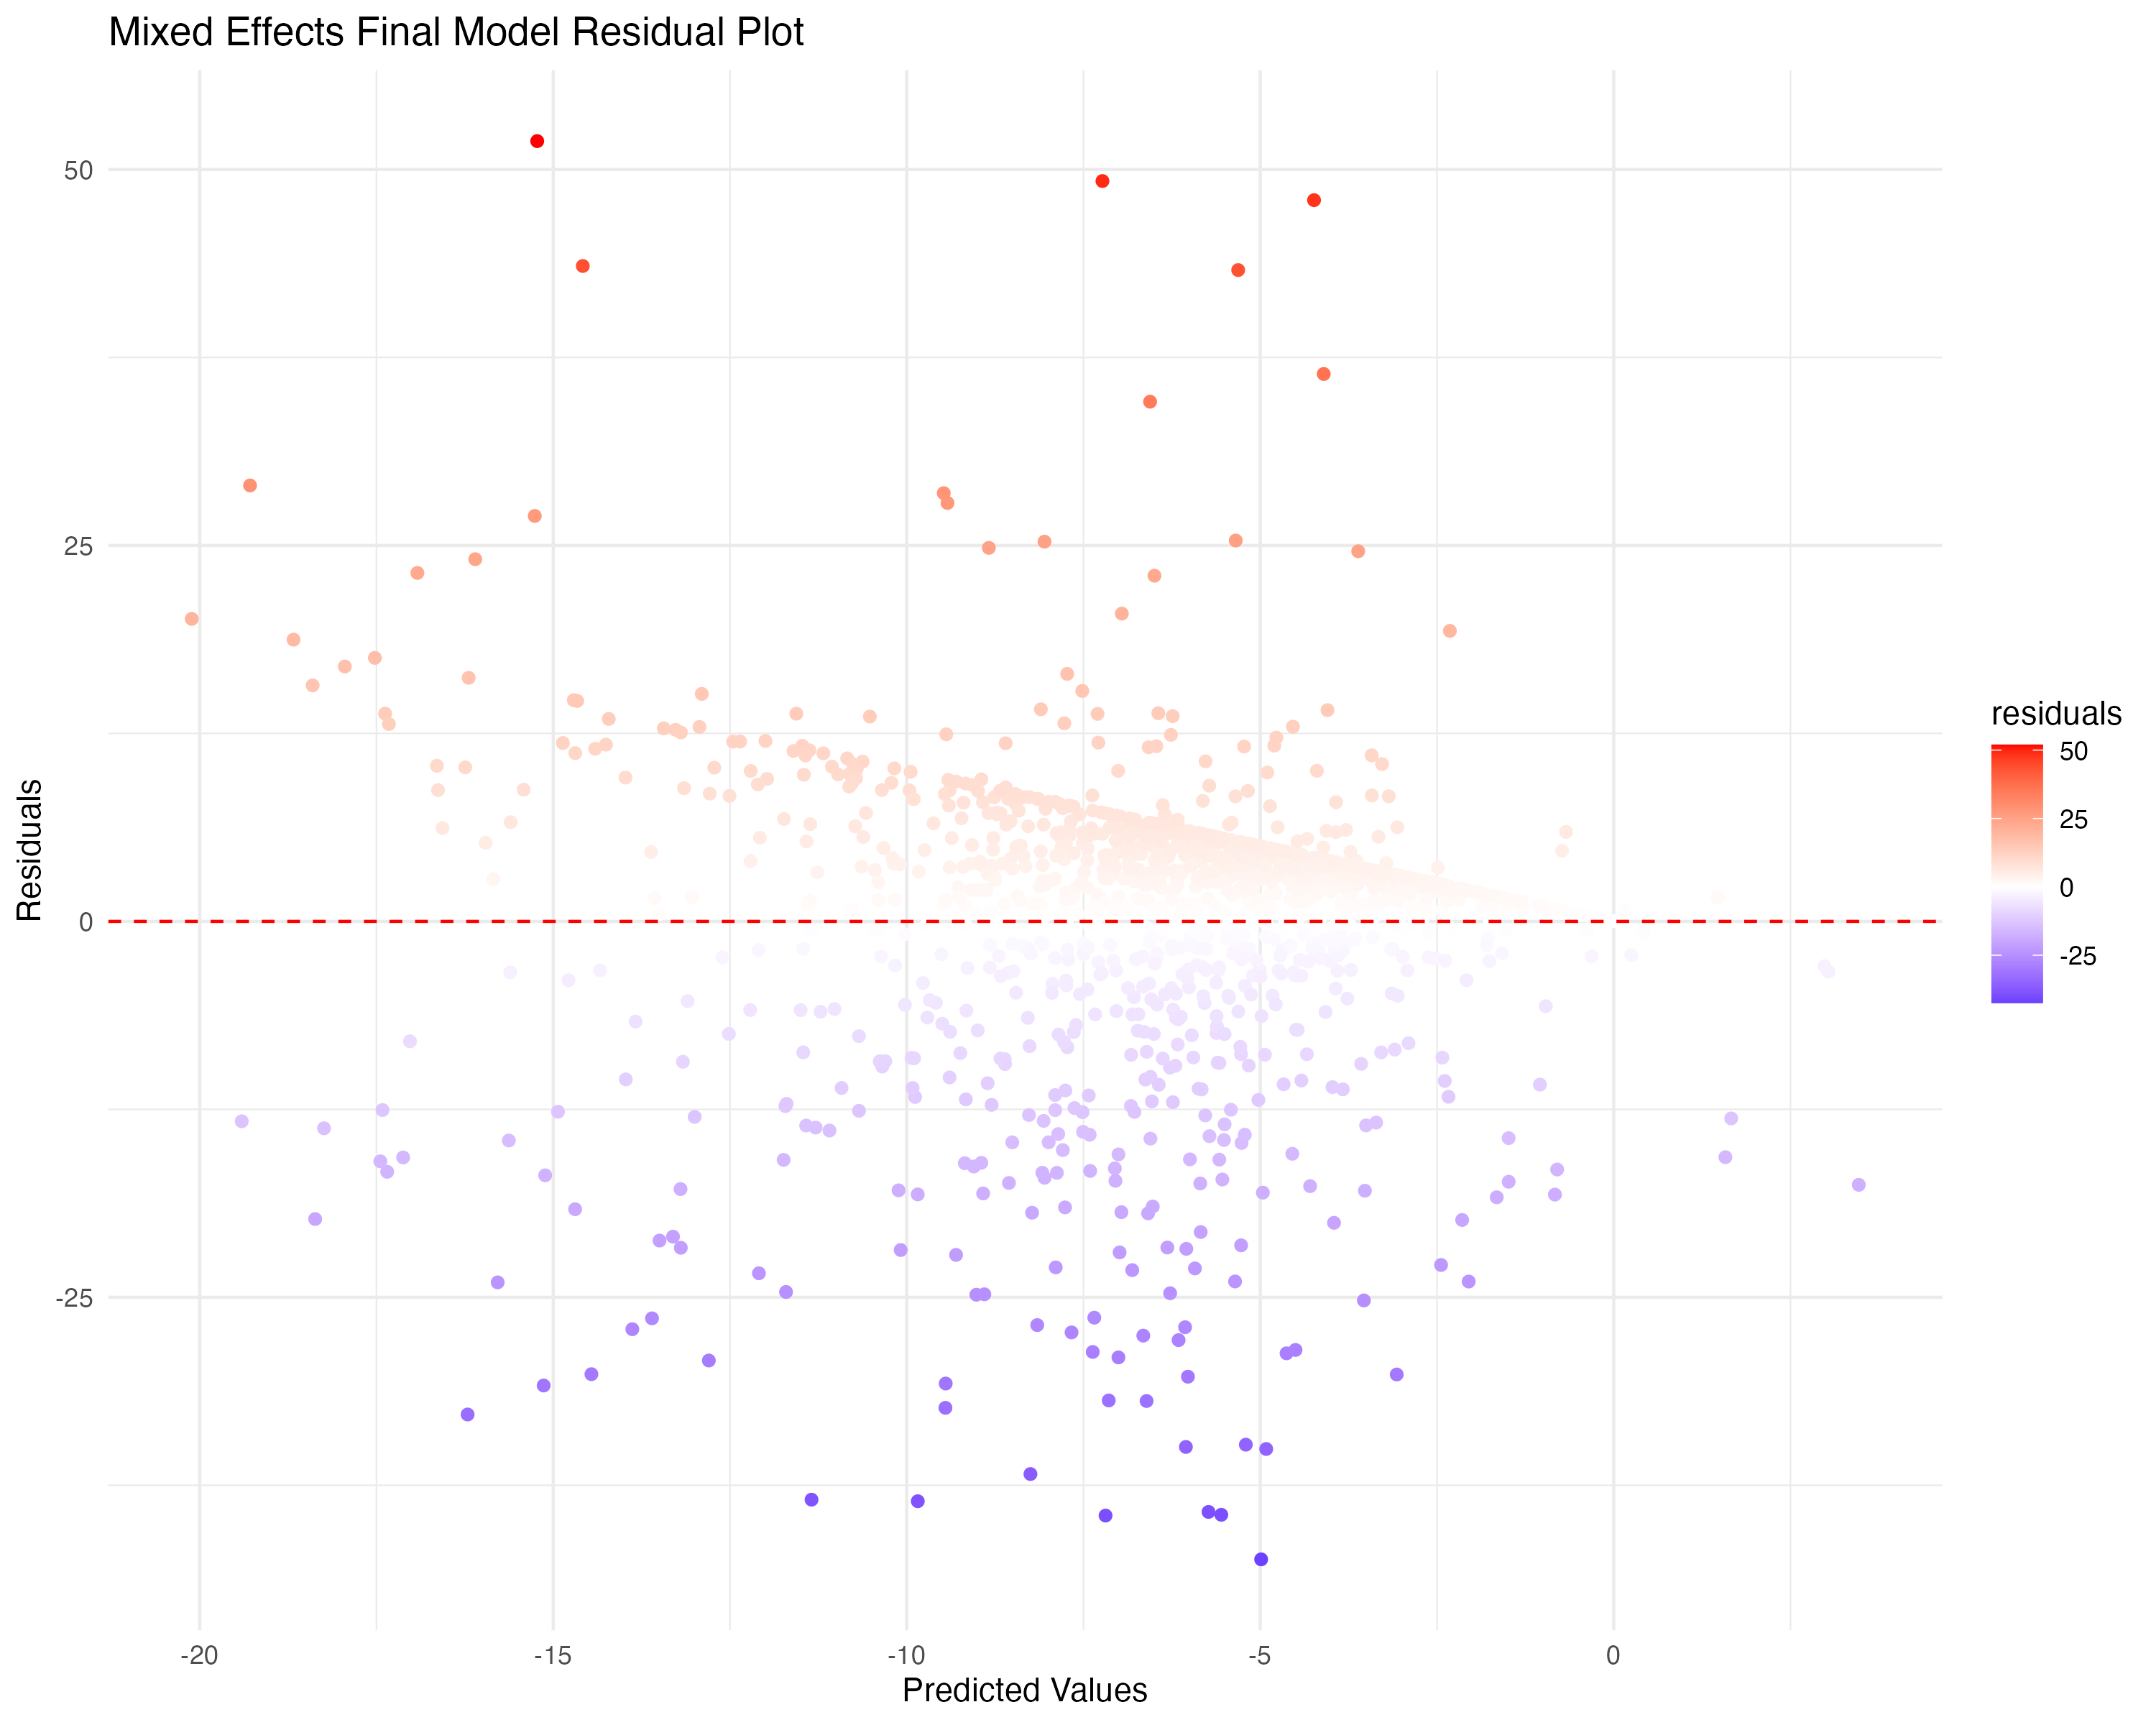
\includegraphics[width=0.8\textwidth]{figures/final_model_residuals.png}
    \caption{Mixed Effects Model (30) Residuals Plot}
    \label{fig:mixed_effects_residuals}
\end{figure}
\noindent The residuals plot is centered around zero, but there are significant outliers, especially for firms with positive change in decarbonization rate and for firms with an absolute change of more than 20\%. Furthermore, we can observe a pronounced diagonal trend, which is likely the due to the presence of zero-inflated data caused by companies failing to report their decarbonization rates when disclosing. This is a major challenge, and it negatively impacts the accuracy of all models, especially because there is no clear imputation method in this case.

\section{Model Selection and Benchmarking}
Using Pycaret \cite{pycaret}, a Machine Learning library, we will be comparing the performance of various models on the dataset. The models will be evaluated based on the RMSE, MAE, and R-squared values. The best model will be selected based on the RMSE value. We used timeseries cross-validation to ensure that the data is split in a time series fashion. As explained in the introduction, the folds are created using the TimeSeriesSplit method from the scikit-learn library \cite{scikit-learn}. We are not tuning the hyperparameters for the models in this section, as we will be doing that in the next section only for the best model. This analysis is useful in identifying which candidate models perform best on the dataset, and consequently which models are worth tuning.

% include table
\begin{longtable}{lrrrr}
\caption{Cross Validation Results for All Tested Models}
\label{tab:cross-validated-results}\\
\toprule
                          Model &   MAE &     MSE &  RMSE &     R2 \\
\midrule
\endfirsthead
\caption[]{Cross Validation Results for All Tested Models} \\
\toprule
                          Model &   MAE &     MSE &  RMSE &     R2 \\
\midrule
\endhead
\midrule
\multicolumn{5}{r}{{Continued on next page}} \\
\midrule
\endfoot

\bottomrule
\endlastfoot 
% color 6.91 green
                 Bayesian Ridge &  4.15 &   48.40 &  \textbf{6.91} &   0.09 \\
             CatBoost Regressor &  4.34 &   48.77 &  6.94 &   0.09 \\
               Ridge Regression &  4.22 &   48.74 &  6.94 &   0.08 \\
    Orthogonal Matching Pursuit &  4.29 &   49.09 &  6.96 &   0.08 \\
                    Elastic Net &  4.25 &   49.35 &  6.97 &   0.08 \\
               Lasso Regression &  4.23 &   49.54 &  6.99 &   0.07 \\
   Lasso Least Angle Regression &  4.23 &   49.54 &  6.99 &   0.07 \\
    Gradient Boosting Regressor &  4.34 &   49.57 &  7.00 &   0.07 \\
Light Gradient Boosting Machine &  4.35 &   49.71 &  7.01 &   0.07 \\
        Random Forest Regressor &  4.56 &   50.25 &  7.04 &   0.06 \\
          Extra Trees Regressor &  4.51 &   50.90 &  7.08 &   0.05 \\
                Dummy Regressor &  4.45 &   54.09 &  7.30 &  -0.01 \\
      Extreme Gradient Boosting &  4.85 &   57.20 &  7.51 &  -0.07 \\
          K Neighbors Regressor &  4.80 &   60.37 &  7.71 &  -0.13 \\
                Huber Regressor &  4.38 &   67.05 &  8.13 &  -0.25 \\
        Decision Tree Regressor &  5.89 &   96.97 &  9.80 &  -0.84 \\
             AdaBoost Regressor &  9.13 &  115.14 & 10.60 &  -1.12 \\
   Passive Aggressive Regressor &  6.84 &  187.64 & 12.92 &  -2.66 \\
              Linear Regression & 31.33 & 3024.39 & 35.90 & -42.10 \\
\end{longtable}


\noindent Note how Bayesian Ridge and CatBoost have the lowest RMSE values. Our intuition in the Methods chapter is supported by this cross-validation exercise. We will be exploring these models further in the next section. In general though, note how no model is significantly better than the others, which suggests that there is significant unexplained variance in the data. This is to be expected, as the CDP survey data is a first step in understanding the decarbonization rate, but there are many other factors that determine decarbonization, especially in the long term. Additionally, there is significant noise in the data due to inconsistent reporting, which makes it difficult to predict the decarbonization rate accurately for any given firm. 

\section{Bayesian Ridge Model}

The Bayesian Ridge model is a linear regression model that uses a Bayesian approach to estimate the coefficients. We defined the model in Chapter \ref{ch:methods}. The hyperparameters that we tuned are the alpha parameter, which controls the strength of the regularization, and the lambda parameter, which controls the strength of the prior distribution on the coefficients. The best model was selected based on the RMSE value. Train and test results are reported in the Table \ref{tab:bayesian_ridge_performance} below. 

\begin{table}[H]
    \centering
    \caption{Bayesian Ridge Model Performance Metrics}
    \label{tab:bayesian_ridge_performance}
    \begin{tabular}{lcccc}
    \hline
    Set & $R^2$ & RMSE & MSE & MAE \\ 
    \hline
    Training & 0.9 & 6.91 & 48.4 & 4.15 \\
    Test & 0.10 & 9.59 & 91.9 & 6.46 \\
    \hline
    \end{tabular}
\end{table}
\noindent The Bayesian Ridge model has a RMSE of 9.59 on the test set, which is very similar to the Mixed Effects Model. This suggests that the Bayesian Ridge model is not significantly better than the Mixed Effects Model. 

\subsection{Feature Importance Plot}
% Feature Importance Plot
\begin{figure}[H]
    \centering
    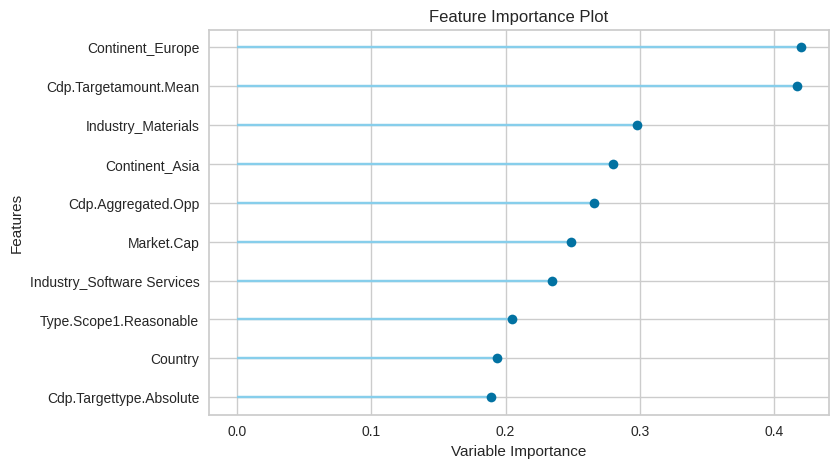
\includegraphics[width=0.6\textwidth]{figures/Bayes_Importance.png}
    \caption{Bayesian Ridge Model Feature Importance Plot}
    \label{fig:bayesian_ridge_feature_importance}
\end{figure}
The feature importance plot \ref{fig:bayesian_ridge_feature_importance} shows that the most important features are continent Europe, the Target Amount Mean, the industry Materials, whether the firm identified an opportunity to reduce emissions. All those features are consistent with the Mixed Effects Model and the Exploratory Data Analysis we performed in Chapter \ref{ch:data-sources}. 

\subsection{Residuals Plot}
% Residuals Plot
\begin{figure}[H]
    \centering
    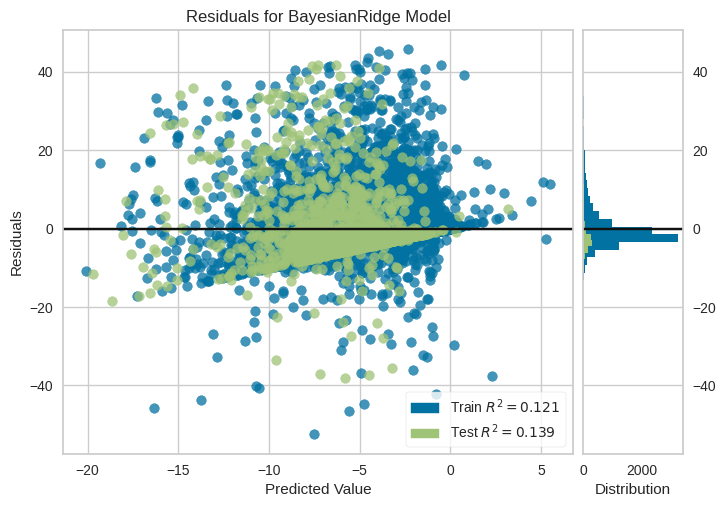
\includegraphics[width=0.8\textwidth]{figures/Bayes_Residuals.png}
    \caption{Bayesian Ridge Model Residuals Plot}
    \label{fig:bayesian_ridge_residuals}
\end{figure}

The residuals plot is similar to the Mixed Effects Model, centered around zero, but with significant outliers, especially for firms with positive change in decarbonization rate and for firms with an absolute change of more than 20\%. This suggests that both models have similar performance and are not performing well for these firms. This makes sense and is consistent with the fact that the data is noisy and that with a greater focus on enhancing reporting quality for decarbonization rates, as we suggest Chapter \ref{chap:conclusion}, the models could be greatly improved. Note how also here we find a significant diagonal trend in the test set, also likely to be caused by zero-inflated data due to companies not reporting their decarbonization rates.

\section{CatBoost Regressor Model}
To tune the CatBoost Regressor model, we used grid search and cross-validation to find the best hyperparameters for the model. The hyperparameters that we tuned are the learning rate, the depth of the tree, the number of trees, and the l2 regularization parameter. We used the TimeSeriesSplit method from the scikit-learn library to ensure that the data is split in a time series fashion with number of folds $cv = 3$. The best model was selected based on the RMSE value. The specific hyperparameters' values that we tuned are reported below:

\begin{table}[H]
    \centering
    \caption{Hyperparameters for CatBoost Regressor}
    \label{tab:hyperparameters}
    \begin{tabular}{@{}lcc@{}}
    \toprule
    Parameter       & Grid of Values        & Selected Best Value \\ 
    \midrule
    Depth           & 4, 6, 8               & \textbf{6}                   \\
    Iterations      & 500, 1000             & \textbf{1000}                \\
    Learning Rate   & 0.01, 0.02, 0.03      & \textbf{0.02}                \\
    L2 Leaf Reg     & 1, 3                  & \textbf{1}                   \\ 
    \bottomrule
    \end{tabular}
\end{table}



\subsection{Model Performance Metrics}
\begin{table}[H]
    \centering
    \caption{CatBoost Regressor Tuned Model Performance Metrics}
    \label{tab:CatBoost_regressor_performance}
    \begin{tabular}{lcccc}
    \hline
    Set & $R^2$ & RMSE & MSE & MAE \\ 
    \hline
    Training & 0.33 & 5.73 & 35.91 & 3.47 \\
    Test & 0.11 & 9.54 & 91.13 & 6.25 \\
    \hline
    \end{tabular}
\end{table}
\noindent The CatBoost Regressor model has a RMSE of 9.54 on the test set, and the $R^2$ value is 0.11, which is the best performance so far. This suggests that the CatBoost Regressor model is the best model for this dataset. It does not come as a surprise, as CatBoost is known for its ability to handle categorical variables and its robustness to overfitting. Therefore, model performance is in line with theoretical expectations and the results from the previous chapter with the main takeaway being that the model is able to generalize well to the test set, but the noise in the response variable significantly limits predictive performance.


    

\subsection{Feature Importance Plot}

\begin{figure}[H]
    \centering
    \includegraphics[width=0.8\textwidth]{figures/CatBoost_feature_importance.png}
    \caption{CatBoost Regressor Feature Importance Plot}
    \label{fig:CatBoost_feature_importance}
\end{figure}
\noindent CatBoost has a built-in feature importance plot, which is shown in Figure \ref{fig:CatBoost_feature_importance}. The most important features are the Current Decarbonization Rate Change, Target Amount Mean, Continent, whether the firm reports market based emissions, and the industry. Note how reassuringly all the selected features by a tree-based boosting method, which is very different from the linear models, are consistent with the Mixed Effects Model and the Bayesian Ridge Model. We therefore learn that there is a consensus across models that the most important features are the same, thus to advance our ability to predict the decarbonization rate, we should focus on these features. We will further elaborate on this argument in Chapter \ref{chap:conclusion}.


\subsection{Shapley Beeswarm Values Plot}

\begin{figure}[H]
    \centering
    \includegraphics[width=0.8\textwidth]{figures/CatBoost_shap_values_beeswarm.png}
    \caption{CatBoost Regressor Shapley Beeswarm Values}
    \label{fig:CatBoost_shapley_values}
\end{figure}

In our analysis using the CatBoost Regressor model, we use Shapley values—derived from game theory—to interpret the model's predictions (\cite{NIPS2017_7062}). Shapley values, illustrated in Figure \ref{fig:CatBoost_shapley_values} through a beeswarm plot, represent each feature's distribution and impact on prediction outcomes. Higher positions of Shapley values off the x-axis are indicative of a stronger influence on the prediction direction, similar to interpreting coefficients' magnitude in linear models. This approach reveals important insights: first, a positive change in the current decarbonization rate significantly forecasts an increase in the next year’s rate - analogously to what we found in the Mixed Effect Model (30). Analogously, a higher target amount mean correlates with an anticipated improvement in the subsequent year's decarbonization rate. Similarly, the findings for Scope 2 Market Emissions align with those from the Mixed Effects Model (30) as well, indicating that firms reporting market-based emissions are likely to achieve a better decarbonization rate in the following year.





